\chapter{Collektive: aggregate programming in pure Kotlin}\label{chapter:collektive}
The name given to the project is \textbf{Collektive}, which emphasize the aggregate programming aim to dispose of numerous devices that work together to achieve a certain goal. Moreover, the name contains \textbf{kt} to refer to the development in Kotlin.

The goal of Collektive is to provide to the user a minimal DSL that makes it possible to create aggregate programs transparently. It is necessary to keep in mind that the solution needs to respect these requirements:
\begin{itemize}
    \item \textbf{Transparency}: refers to the clear and concise information it provides about how the underlying system behaves, such as data processing, storage, and communication between nodes. Transparency helps to reduce complexity, making it easier to understand and maintain large and complex systems;
    \item \textbf{Minimality}: designing it with the fewest possible constructs and abstractions while still offering the required functionality. This reduces the complexity of the system, making it easier to maintain and debug, and lowers the overhead associated with using the DSL, which is particularly important for systems that require high performance and scalability;
    \item \textbf{Portability}: refers to its ability to run on various platforms and environments, including different operating systems, cloud platforms, and hardware architectures. This enables systems built with the DSL to be easily deployed and run in different environments, which is crucial for systems requiring deployment in multiple locations or scalability to meet changing demands.
\end{itemize}

The following sections are organized in order to present in details the project developed. Specifically, Section \ref{section:technology_choices} discuss the main technological choice involved in the development of the DSL, in Section \ref{section:project_structure} is shown the project structure, in Section \ref{section:dsl} is analyzed in details the DSL created. Then, Section \ref{section:usage_example} presents the final result and how the DSL can be used, and Section \ref{section:validation} is used to highlight the validation methods applied to test the correct behavior of the project developed.

\section{Technology}\label{section:technology_choices}
This section presents the main technological choice taken regarding the development of the DSL, in order to achieve the requirements cited previously.\newline
It is important to achieve a certain level of portability, specifically for devices running on JVM, JS and Kotlin Native platforms, which makes possible also to gain interoperability between different targets. Moreover, an ideal solution would not require writing the DSL code in three different programming languages to match the required platforms.\newline
For the reasons just presented, the choice made for this project development is \textbf{Kotlin Multiplatform}.

\subsection{Kotlin Multiplatform}
Kotlin Multiplatform technology is specifically designed to streamline the development process for cross-platform projects.\newline
It achieves this by minimizing the amount of time developers spend writing and maintaining identical code for different platforms. This approach saves valuable resources and time, as the code can be written once and used across multiple platforms.

Kotlin Multiplatform allows to write code in the Kotlin programming language and use it across multiple platforms, including Android, iOS, web, and desktop.
\begin{figure}[!ht]
    \centering
    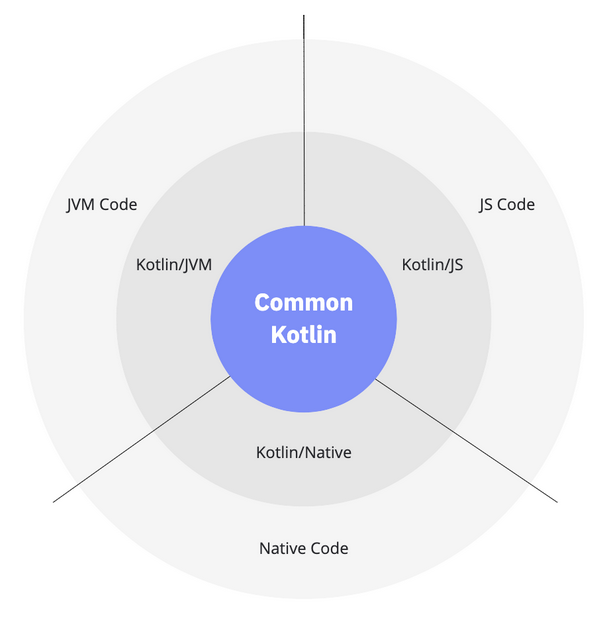
\includegraphics[scale=0.9]{document/chapters/4-collektive/images/kotlin_multiplatform_code.png}
    \caption{How Kotlin Multiplatform works \cite{kotlin_multiplatform_overview}}
    \label{fig:km_code_work}
\end{figure}
As can be seen in Figure \ref{fig:km_code_work}, Kotlin Multiplatform code behaves in the following way \cite{kotlin_multiplatform_overview}:
\begin{itemize}
    \item \textbf{Common Kotlin}: the code written in common Kotlin can be used across multiple platforms without requiring modifications. This code can include business logic, data models, and other non-platform-specific functionality. Common code can rely on a set of libraries that are available for Kotlin Multiplatform and that cover everyday tasks, such as serializations or coroutines;
    \item \textbf{Platform-specific versions of Kotlin}: this refers to \textbf{Kotlin/JVM}, \textbf{Kotlin/JS} and \textbf{Kotlin/Native}, which include extensions to the Kotlin language, allowing developers to use platform-specific APIs, features and tools;
    \item \textbf{Platform native code}: finally, through these platforms it is possible to access the platform native code (JVM, JS and Native), with the possibility to use all the native features.
\end{itemize}

The way that Kotlin Multiplatform avoid the necessity to write and maintain the same code over and over again for all the targeted platforms, is by providing the possibility to share the same code across multiple platforms.\newline
It is possible to share the code in different ways \cite{kotlin_multiplatform_share_code}:
\begin{itemize}
    \item \textbf{Share code on all platforms}: this is typically done when some business logic is common to all platforms, in order to write it only once in the common code and then share it on all the targets, as shown in Figure \ref{fig:km_share_code_on_all_platforms};
    \begin{figure}[!ht]
        \centering
        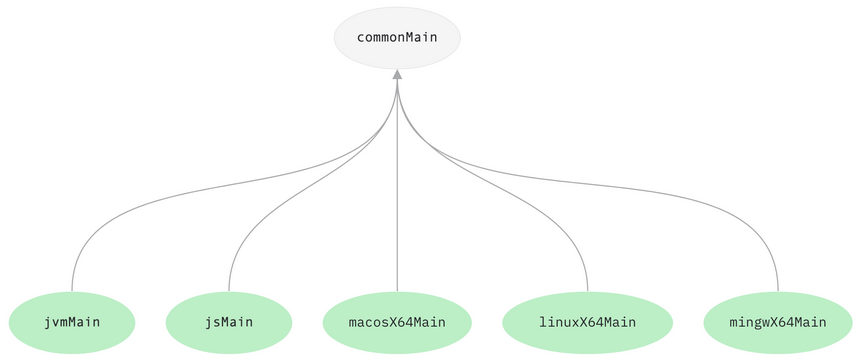
\includegraphics[scale=0.86]{document/chapters/4-collektive/images/km_share_code_on_all_platforms.png}
        \caption{Kotlin Multiplatform used to share code on all platforms \cite{kotlin_multiplatform_share_code}}
        \label{fig:km_share_code_on_all_platforms}
    \end{figure}
    \item \textbf{Share code among some platforms}: this organization is usually applied when similar platforms share a big portion of code. As it can be seen in Figure \ref{fig:km_reuse_code}, it is possible to define hierarchies that allow to organization the share code, such as the \textit{desktopMain} folder that shares only define some shared code for its dependencies.
    \begin{figure}[!ht]
        \centering
        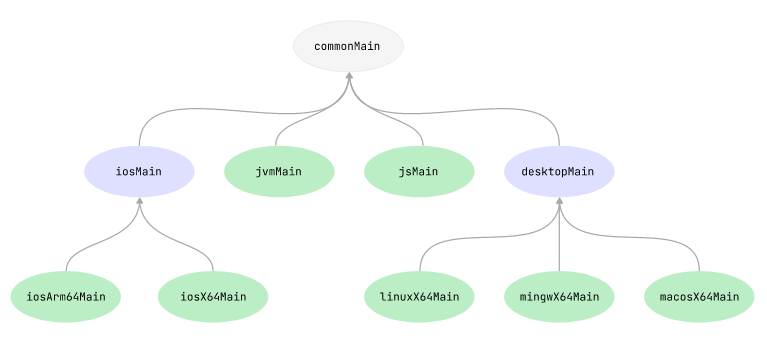
\includegraphics[scale=0.97]{document/chapters/4-collektive/images/kotlin_multiplatform_reuse_code.png}
        \caption{Kotlin Multiplatform reuse of code among some platforms of the project \cite{kotlin_multiplatform_overview}}
        \label{fig:km_reuse_code}
    \end{figure}
\end{itemize}

In some cases it might be necessary to access platform-specific APIs from the common code. This can be done by using the specific Kotlin mechanism of expected and actual declarations \cite{kotlin_multiplatform_expect_actual}.\newline
\begin{figure}[!ht]
    \centering
    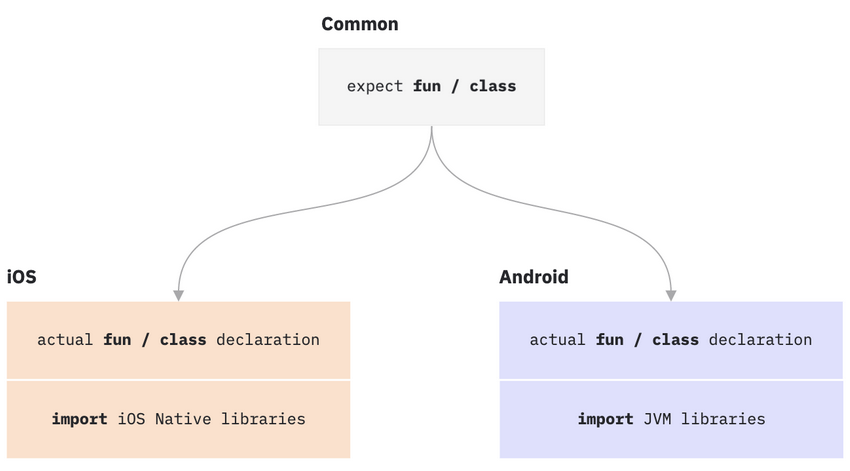
\includegraphics[scale=0.85]{document/chapters/4-collektive/images/km_expect_actual.png}
    \caption{Kotlin Multiplatform expect and actual dependency mechanism \cite{kotlin_multiplatform_expect_actual}}
    \label{fig:km_expect_actual}
\end{figure}
In Figure \ref{fig:km_expect_actual} it is shown an example of this mechanism. For instance, in the common code it is created a new function or class, and it is declared using the keyword \textbf{expect}. The keyword informs the compiler that it should look for the implementation of this element in the platform-specific folders. This can be done by declaring the same function or class by using the \textbf{actual} keyword, which allows taking advantage of specific APIs. In the cited example, the actual implementation required are for the iOS and Android platforms.

Kotlin Multiplatform also includes tools to help developers manage their codebase, such as Gradle plugins that allow for building and testing code across multiple platforms.

One advantage of Kotlin Multiplatform is, for example, the ability to share code between Android and iOS. This can be especially valuable for companies that want to develop apps for both platforms, as it can help reduce development time and costs. With Kotlin Multiplatform, developers can write shared code for common features, such as user authentication or data storage, and then write platform-specific code for the UI and other platform-specific features.

Concluding, Kotlin Multiplatform is the perfect technology to achieve this thesis project, because it allows creating a unique code base that is possible to use on three different platforms: JVM, JavaScript and Native. Moreover, it is not required the implementation of platform-specific behaviors, meaning that one the common code has been developed.

\section{Project structure}\label{section:project_structure}
Collektive has been developed as a Gradle project composed by three different submodules, as shown in Figure \ref{fig:collektive_package_diagram}:
\begin{enumerate}
    \item \textbf{plugin}:
    \begin{enumerate}
        \item \textbf{gradle-plugin}:
        \item \textbf{compiler-plugin}:
    \end{enumerate}
    \item \textbf{dsl}:
    \item \textbf{collektive-test}:
\end{enumerate}
\begin{figure}[!ht]
    \centering
    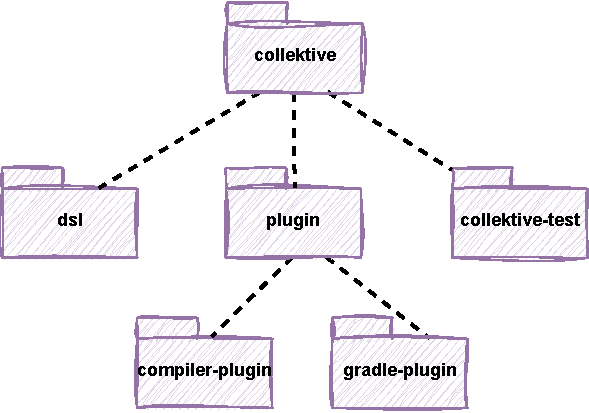
\includegraphics[scale=1.1]{document/chapters/4-collektive/images/collektive_package_diagram.pdf}
    \caption{Package diagram of Collektive project}
    \label{fig:collektive_package_diagram}
\end{figure}

\section{DSL}\label{section:dsl}
A \textbf{DSL} (Domain-Specific Language) \cite{dsl_definition} is a programming language or language construct that is designed to be highly specific to a particular domain, or problem space. Unlike general-purpose programming languages, which are intended to be applicable across a wide range of domains and problem types, DSLs are created to meet the specific needs of a particular application or system. For this reason, general-purpose languages, such as Java, are generally more complex than DSL.\newline 
DSLs can be implemented in a number of ways, including as standalone programming languages, as libraries that extend existing programming languages, or as annotations or macros that modify the syntax or behavior of an existing language. DSLs can be used to provide a higher level of abstraction over complex systems or processes, allowing developers to express ideas and concepts in a more concise and intuitive way.\newline
To ensure that DSLs are fit for their intended purpose, they are typically developed in close collaboration with domain experts. In fact, many DSLs are not designed to be used by programmers, but rather by non-technical individuals who are knowledgeable in the relevant domain. This collaborative approach helps to ensure that the DSL is intuitive and expressive for its intended users, allowing them to more easily and effectively express complex ideas and processes.

\section{Usage examples}\label{section:usage_example}

\section{Validation}\label{section:validation}
